\section{Results}

\subsection{Histograms}

\begin{figure}[H]
    \centering
    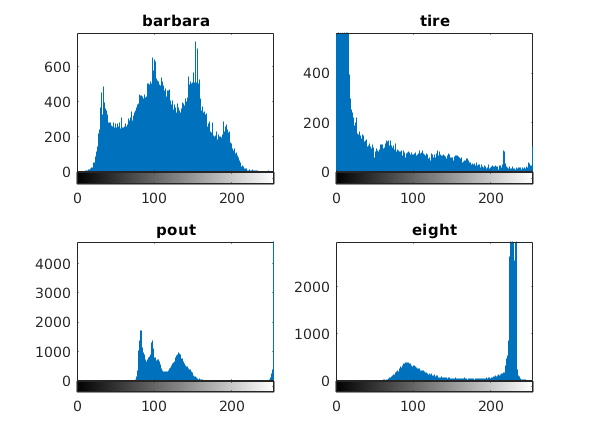
\includegraphics[scale=0.75]{histogram_compare.png}
    \caption{Histograms of Several Images}
\end{figure}

Barbara has a concentration of intensities in the middle, however has very few
at the minimum and maximum values. Tire spans the entire range of intensities,
but has a massive concentration at very dark levels. Pout has very concentrated
values around middle intensity levels, this will result in very low contrast.
Finally, eight has some values in the mid-range, but has a very large
concentration of intensity at high levels. Overall I expect tire to be the
darkest image and eight to be the brightest.

\subsection{Histogram Equalization}


\begin{figure}[H]
    \centering
    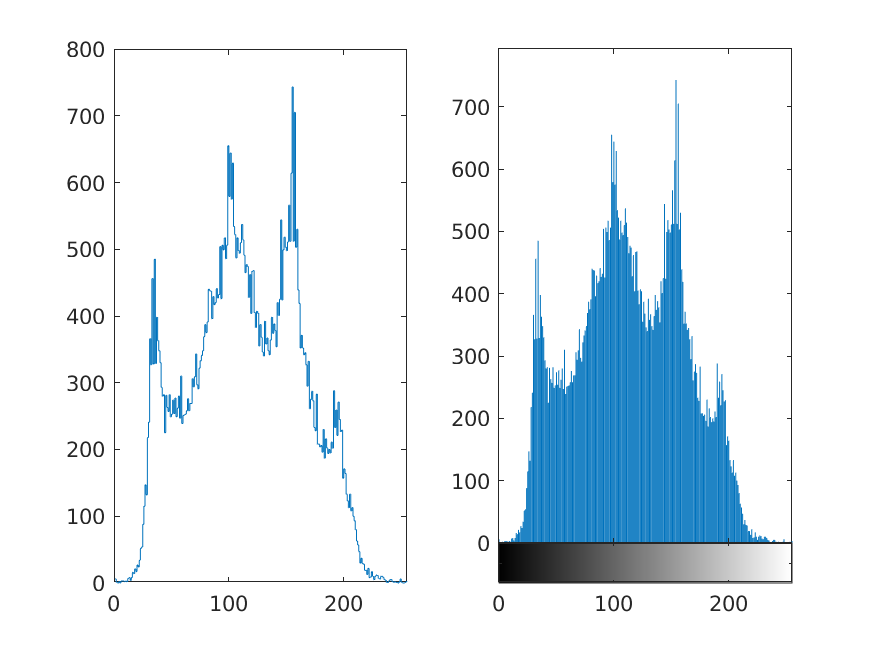
\includegraphics[scale=0.75]{barbara_compare.png}
    \caption{My histogram function vs. imhist of barbara}
\end{figure}

\begin{figure}[H]
    \centering
    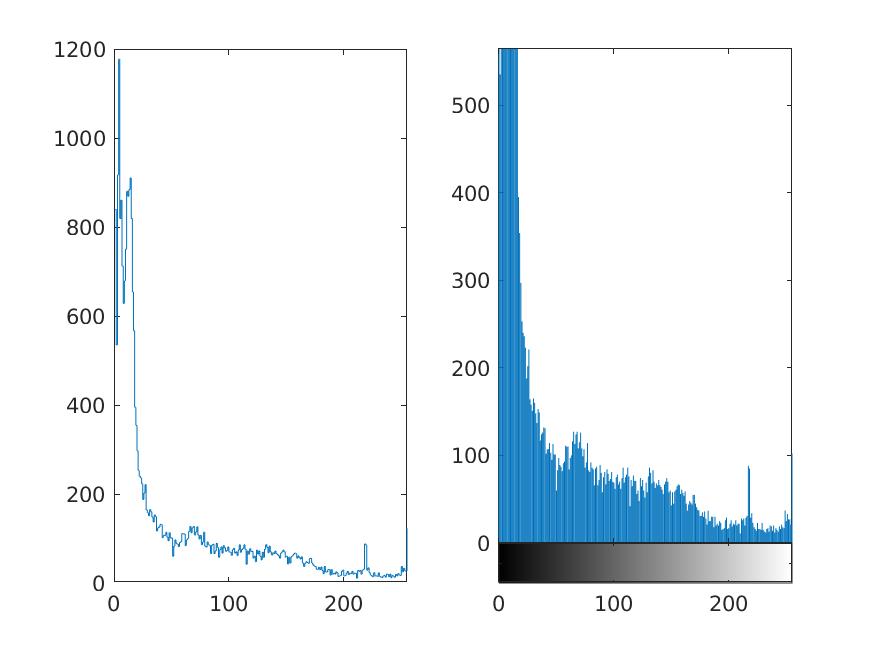
\includegraphics[scale=0.75]{Tire_gray_compare.png}
    \caption{My histogram function vs. imhist of Tire\_gray}
\end{figure}

\begin{figure}[H]
    \centering
    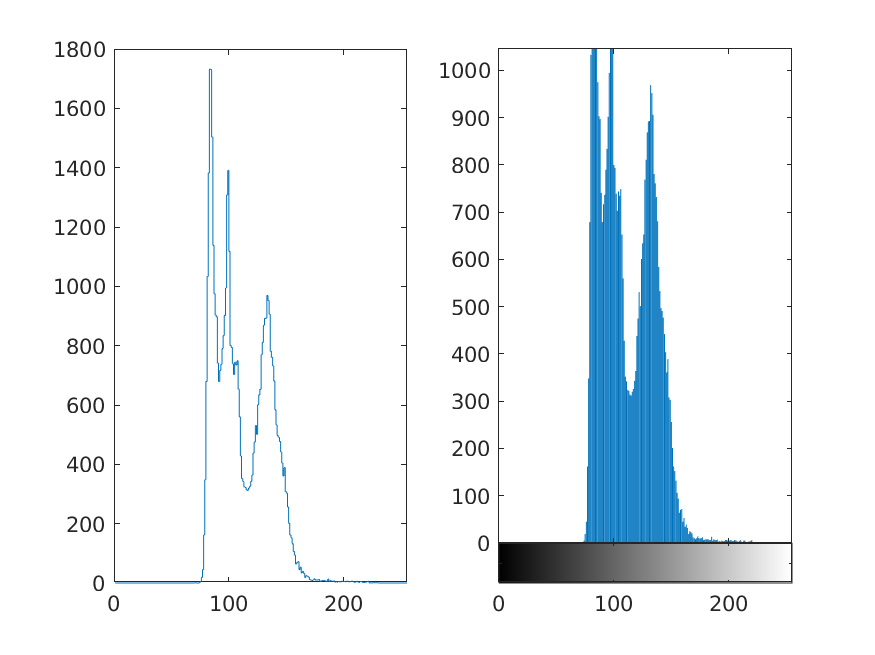
\includegraphics[scale=0.75]{pout_gray_compare.png}
    \caption{My histogram function vs. imhist of pout\_gray}
\end{figure}

\begin{figure}[H]
    \centering
    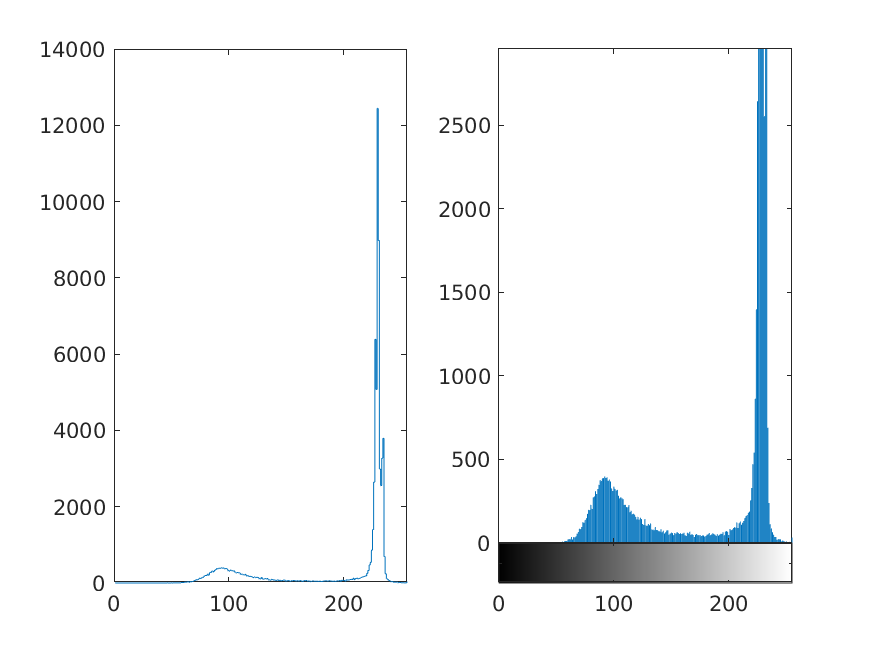
\includegraphics[scale=0.75]{eight_gray_compare.png}
    \caption{My histogram function vs. imhist of eight\_gray}
\end{figure}

First I've tested my histogram function on our images. While the Matlab function
adds in some pretty plotting stuff, I have clearly scripted my function
correctly. In some cases it seems that Matlab cuts off view of some intensities
and in my plots you can see how many pixels there really are for a given
intensity.

\begin{figure}[H]
    \centering
    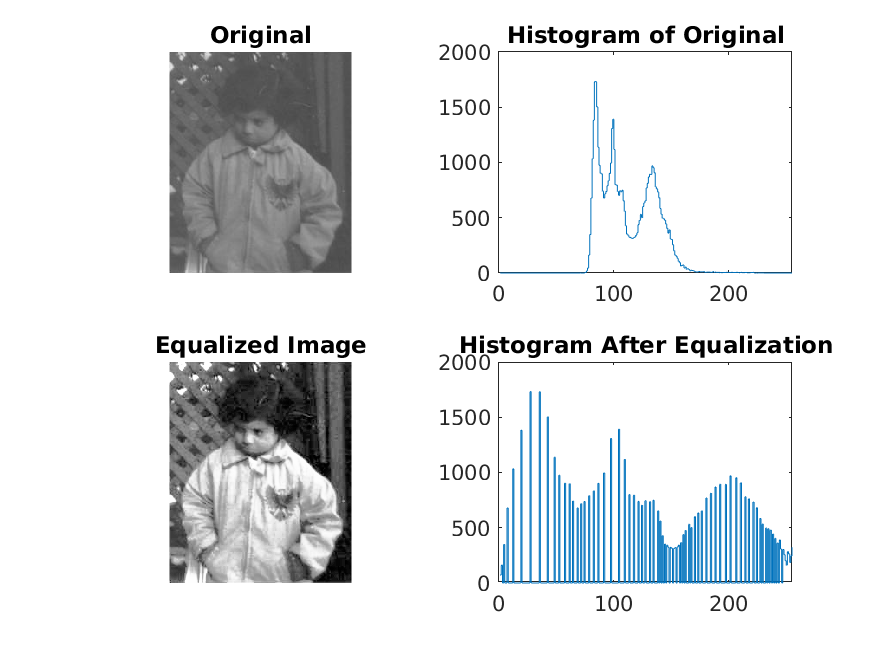
\includegraphics[scale=0.75]{pout_gray_equalize.png}
    \caption{Histogram Equalization of pout}
\end{figure}

\begin{figure}[H]
    \centering
    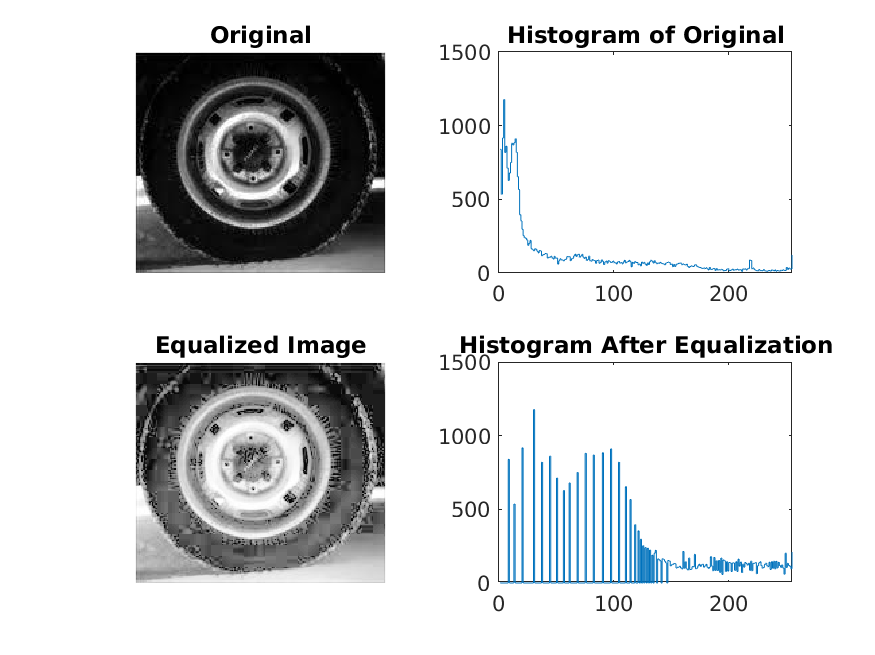
\includegraphics[scale=0.75]{Tire_gray_equalize.png}
    \caption{Histogram Equalization of Tire}
\end{figure}

I've used histogram equalization in the above two images and showed the
histogram and image before and after the equalization. You can see the
histograms for both images expand as they are equalized. Visually, pout was
greatly enhanced, and looks better. Tire however does not look visually
pleasing. The contrast has expanded, but it seems to have moved lower
intensities into higher regions where pout's intensities moved from center
intensities to both high and low intensities. I can see equalization being
heavily used in the enhancement of old photos.

\subsection{Histogram Matching}
